\chapter{Results}

\section{Overhead}

One of our first concerns was to implement a framework that does not impact to our simple application.
The benchmarking framework shoul be hidden for the developer.
Enabling the framework should not altering the good use of the application.

To mesure the impact of our approaches, we used the same setup than with our reference value and retrieve 1000 measurements of the context switching time.
We compared those measurements with our reference value and compute the overhead of our framework.
The oscilloscope measurements are shown in the figure \ref{fig:overhead-reference-value-contiki-z1}.

\subsection{Extension approach overhead}

The extension approach have a large overhead of more than 2ms for with RE-Mote board and more than 3ms with the Z1 board on both Contiki and RIOT.
On the figure \ref{fig:overhead-extension-contiki-z1}, we can see the overhead of the first approach with the measurements made by the oscilloscope.
We discuss later why our extension approach add such a latency in the section \ref{sec:overhead}.

\subsection{Devices approach overhead}

The devices approach, in the other hand, have a small overhead of less than $3\mu s$ with either the RE-Mote or the Z1 boards on both Contiki and RIOT.
On the figure \ref{fig:overhead-devices-contiki-z1}, we can see the overhead of the devices approach.
The devices approach add a much more smaller overhead to our simple application than the extension approach.
This difference between the overhead of the two approaches is discussed in the section \ref{sec:overhead}.

\begin{figure}[!ht]
        \centering
        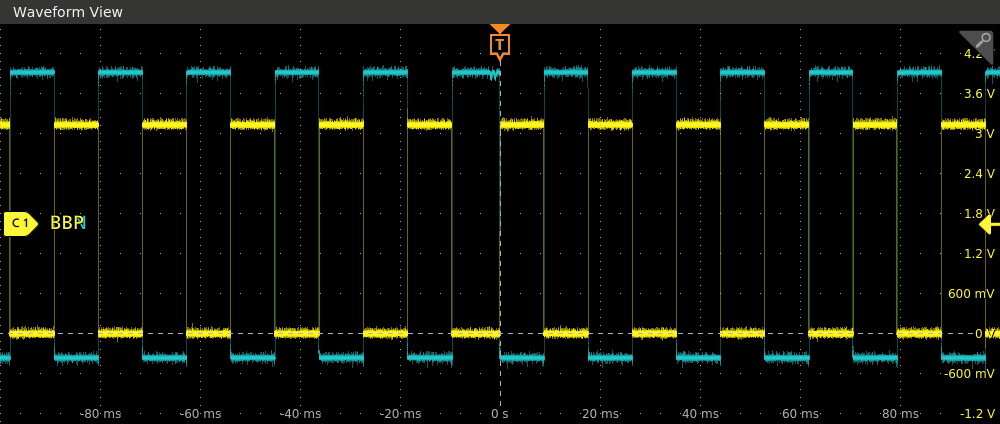
\includegraphics[scale=.4]{assets/reference-value-overhead-contiki-z1.png}
        \caption{overhead reference measured by the oscilloscope\label{fig:overhead-reference-value-contiki-z1}}

        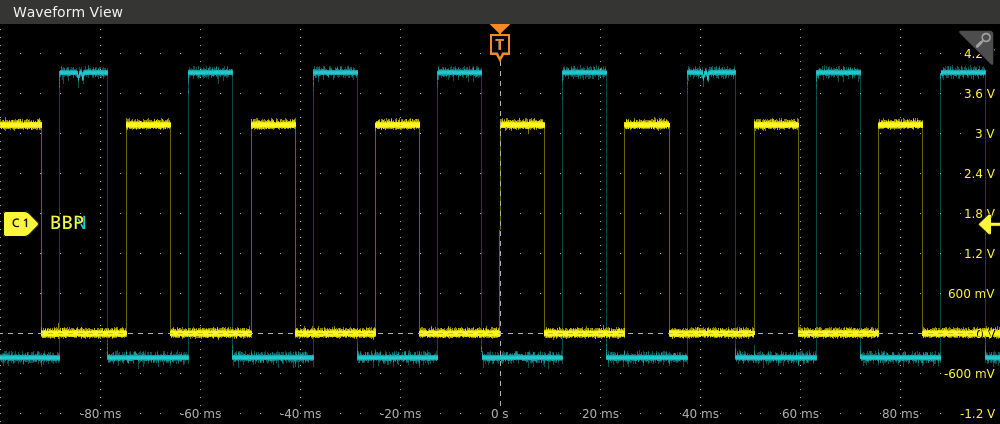
\includegraphics[scale=.4]{assets/extension-framework-overhead-contiki-z1.png}
        \caption{extension approach overhead measured by the oscilloscope\label{fig:overhead-extension-contiki-z1}}

        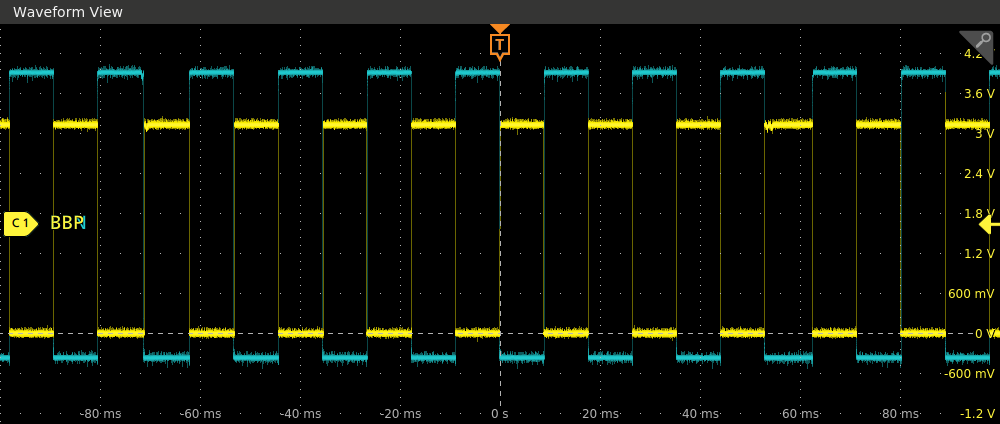
\includegraphics[scale=.4]{assets/devices-framework-overhead-contiki-z1.png}
        \caption{devices approach overhead measured by the oscilloscope\label{fig:overhead-devices-contiki-z1}}
\end{figure}

\section{Framework measurements}

We describe in this section the results gathered with the extension approach described in the section \ref{sec:extension} and with the devices approach described in the section \ref{sec:external}.
For recall, the first approach is to implement the framework as a RTOS module used in the user space and that will compute internally the context switching time.
The second approach is to measure the context switching time using an external board, the PSLab.

In the same way as with the reference value, the results are divided by boards.
The measurements made with the RE-Mote boards are first given, then the one made with Z1 board.
The Contiki measurements are displayed side-by-side with the RIOT one for more clarity.

\subsection{Extension approach measurements}

\subsubsection{RE-Mote board measurements}
With Contiki, the framework outputs measurements with an average of 31.6162 $\mu$s.
With 0$\mu$s as the minimum value and 457.7636 $\mu$s as the maximum value, the measurements have a large distribution.
We have a difference of 13.1112 $\mu$s between the measured context switching time and the real one measured with the oscilloscope.

With RIOT, the framework outputs a constant context switching time of 17 $\mu$s.
All 1000 measurements were equal to 17 $\mu$s.
Thus, the difference with the real context switching time is 4.374 $\mu$s.

Both measurements were above the real context switching time given by the reference value.
The table \ref{tab:extension-framework-remote} shows the measurement for Contiki and RIOT for the RE-Mote board.

\begin{table}[!ht]
  \centering
  \begin{tabular}{l|c|c}
                & Contiki  & RIOT \\ \hline
  Mean ($\mu$s) & 31.6162  & 17      \\
  Min  ($\mu$s) & 0        & 17      \\
  Max  ($\mu$s) & 457.7636 & 17     
  \end{tabular}
  \caption{extension approach measurements for Contiki and RIOT on the RE-Mote board}
  \label{tab:extension-framework-remote}
  \end{table}

\subsubsection{Z1 board measurements}
On the Class-1 Z1 board, the framework gave an average context switching time of 90.5761 $\mu$s with Contiki.
Once again, on Contiki, our values were largely distributed between 30.5175 $\mu$s and 976.5625 $\mu$s.
The average context switching time measured is 35.4991 $\mu$s above the real context switching time.

With RIOT, most of the values were equal to 40 $\mu$s with an average of 40.252 $\mu$s.
This put the measurements 12.553 $\mu$s above the real context switching time.

The table \ref{tab:extension-framework-z1} shows the measurement for Contiki and RIOT for the Z1 board.

\begin{table}[!ht]
  \centering
  \begin{tabular}{l|c|c}
                & Contiki  & RIOT \\ \hline
  Mean ($\mu$s) & 90.5761  & 40.252      \\
  Min  ($\mu$s) & 30.5175  & 40      \\
  Max  ($\mu$s) & 976.5625 & 41     
  \end{tabular}
  \caption{extension approach measurements for Contiki and RIOT on the Z1 board}
  \label{tab:extension-framework-z1}
  \end{table}

\subsection{Devices approach measurement}

\subsubsection{RE-Mote board measurements}
On the RE-Mote board, the devices approach outputs an average context switching time of 19.0329 $\mu$s on Contiki.
This measurement differs from the real context switching time by only 2.85$\%$.
They are 0.5279 $\mu$s above the reference measurements.
The majority of the values were around 14 $\mu$s but some of them were above 40 $\mu$s.
The figure \ref{fig:devices-framework-contiki-remote} show the distribution of the measurements made with Contiki.

\begin{figure}[!ht]
      \centering
      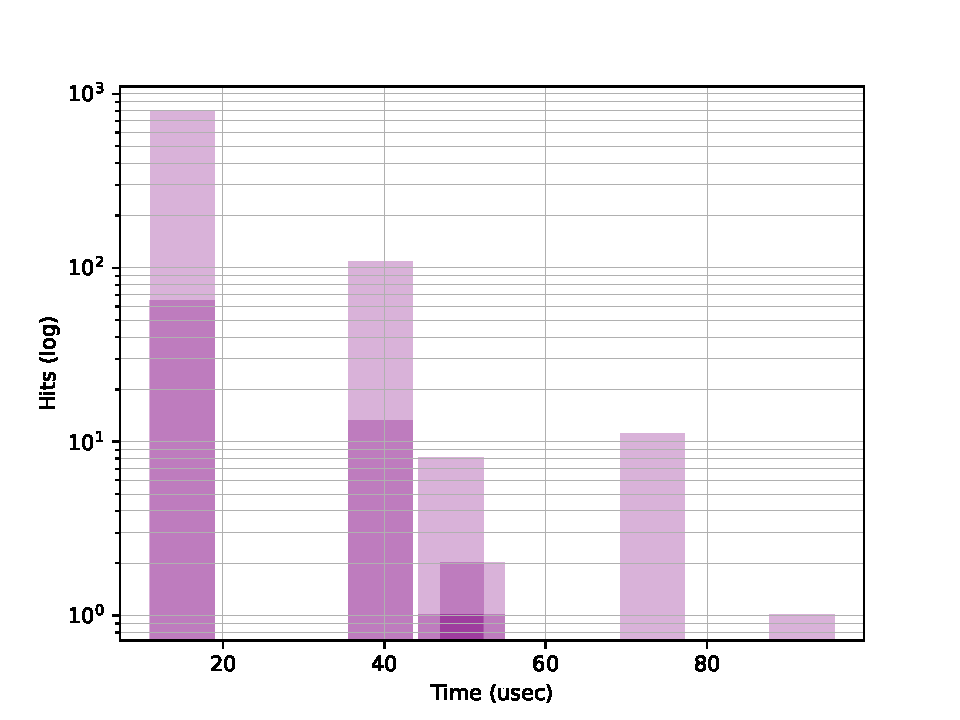
\includegraphics[scale=.7]{assets/devices-framework-contiki-remote.pdf}
      \caption{devices approach measurements distribution with Contiki on the RE-Mote board\label{fig:devices-framework-contiki-remote}}
\end{figure}

With RIOT, the average context switching was 12.9832 $\mu$s.
For RIOT, the measurement were either around 12.95 $\mu$s or around 13 $\mu$s.
The figure \ref{fig:devices-framework-riot-remote} shows this disparity.
The measured context switching time is above the real context switching time by 0.3572 $\mu$s.
This represents an offset of $2.82\%$ from the reference measurements.

\begin{figure}[!ht]
      \centering
      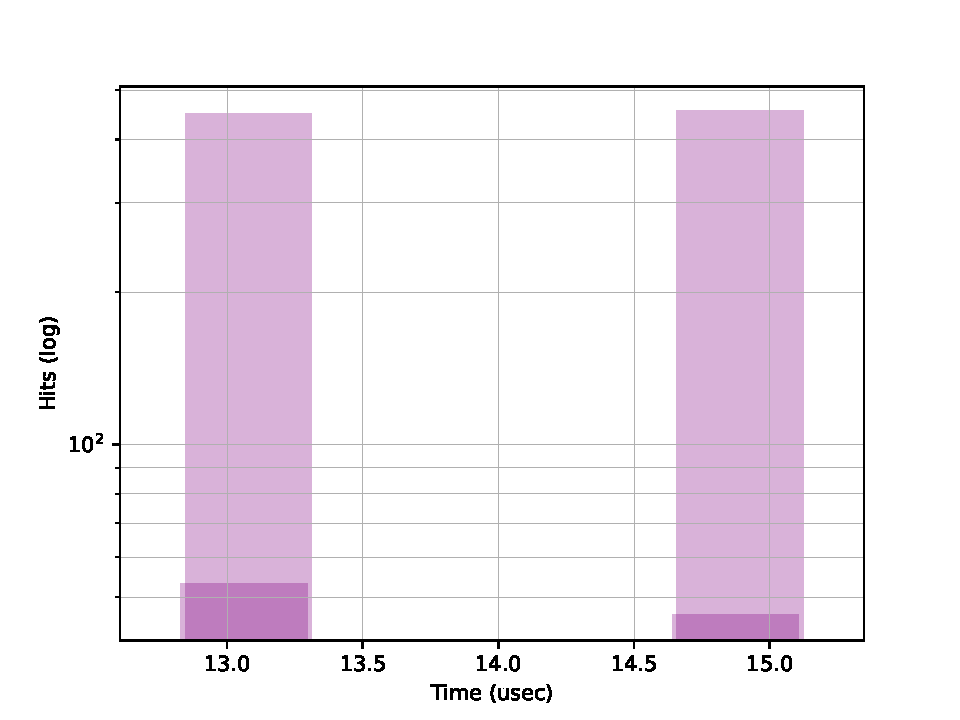
\includegraphics[scale=.7]{assets/devices-framework-riot-remote.pdf}
      \caption{devices approach measurements distribution with RIOT on the RE-Mote board\label{fig:devices-framework-riot-remote}}
\end{figure}

The table \ref{tab:devices-framework-remote} shows the measurement for Contiki and RIOT for the RE-Mote board.

\begin{table}[!ht]
  \centering
  \begin{tabular}{l|c|c}
                & Contiki  & RIOT \\ \hline
  Mean ($\mu$s) & 19.0329  & 12.9823 \\
  Min  ($\mu$s) & 14.9375  & 12.9375 \\
  Max  ($\mu$s) & 91.75    & 13.0156
  \end{tabular}
  \caption{devices framework measurements for Contiki and RIOT on the RE-Mote board}
  \label{tab:devices-framework-remote}
  \end{table}

\subsubsection{Z1 board measurements}
With the second approach, on the Z1 board, the framwork found an average context switching time of 54.99 $\mu$s with Contiki.
The framework measurements were $0.15\%$ off from the real measurements by being 0.087 $\mu$s below them.
However, with Contiki the measured values are more scattered like shown in the figure \ref{fig:devices-framework-contiki-z1}.
The minimum measured context switching time is 32.5625 $\mu$s and the maximum one is 314.5 $\mu$s.

\begin{figure}[!ht]
      \centering
      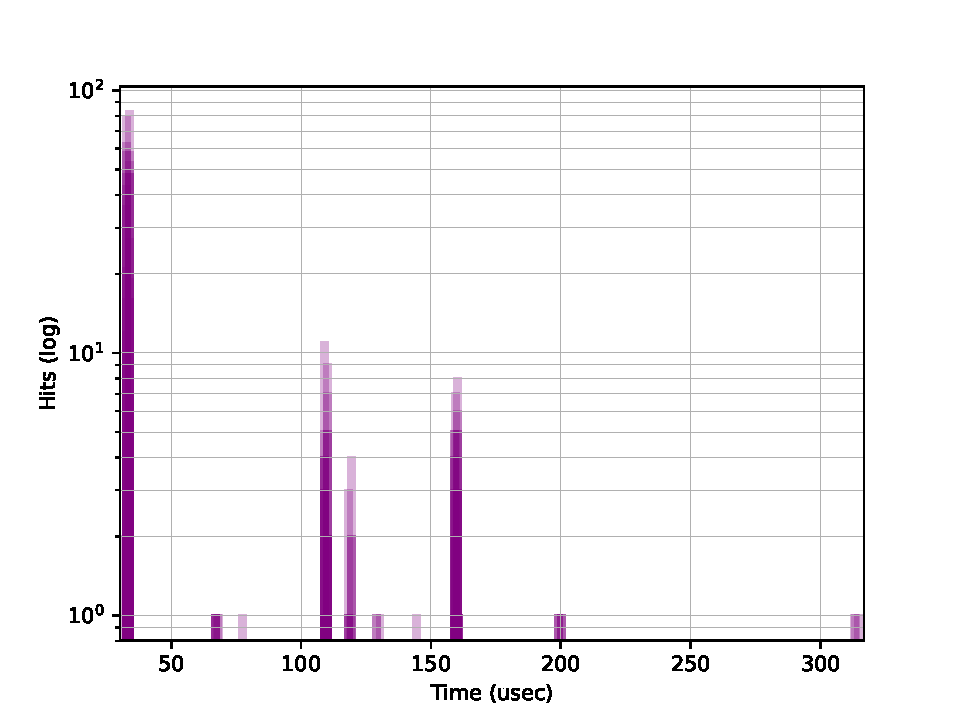
\includegraphics[scale=.7]{assets/devices-framework-contiki-z1.pdf}
      \caption{devices approach measurements distribution with Contiki on the Z1 board\label{fig:devices-framework-contiki-z1}}
\end{figure}

With RIOT, the framework outputted an average context switching time of 30.6971 $\mu$s.
The difference with the real context switching time is 2.9981 $\mu$s making the framework measurements more than $10\%$ above the reference measurements.
On the other hand, the framework measurements gave the same distribution as the one found with the oscilloscope in the section \ref{sec:ref-measurements} with the figure \ref{fig:reference-value-riot-z1}.
The measured measurements distribution is shown in the figure \ref{fig:devices-framework-riot-z1}.

\begin{figure}[!ht]
      \centering
      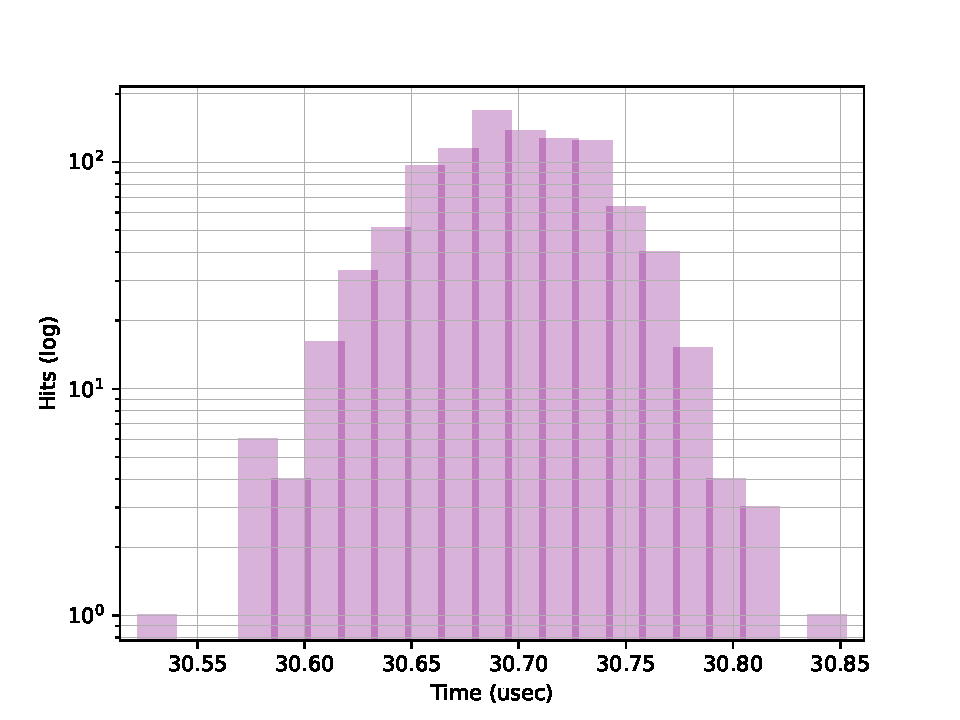
\includegraphics[scale=.7]{assets/devices-framework-riot-z1.pdf}
      \caption{devices approach measurements distribution with RIOT on the Z1 board\label{fig:devices-framework-riot-z1}}
\end{figure}

The table \ref{tab:devices-framework-z1} shows the measurement for both Contiki and RIOT on the Z1 board.

\begin{table}[!ht]
  \centering
  \begin{tabular}{l|c|c}
                & Contiki  & RIOT OS \\ \hline
  Mean ($\mu$s) & 54.99    & 30.6971 \\
  Min  ($\mu$s) & 32.5625  & 30.5312 \\
  Max  ($\mu$s) & 314.5    & 30.8437
  \end{tabular}
  \caption{devices framework measurements for Contiki and RIOT on the Z1 board}
  \label{tab:devices-framework-z1}
  \end{table}

\subsection{Resume}
To give more clarity to the results, the following tables give the average context switching time measured with the two approaches.
The table \ref{tab:framework-measurements-resume-remote} gives the measurements made on the RE-Mote board.
The table \ref{tab:framework-measurements-resume-z1} gives the measurements made on the Z1 board.
The difference between the measured context switching time and the real context switching time measured with the oscilloscope is written between parenthesis.

\begin{table}[!ht]
  \centering
  \begin{tabular}{l|c|c}
                      & Contiki           & RIOT             \\ \hline
  Extension approach ($\mu s$) & 31.6162 (13.1112) & 17 (4.374)       \\
  Devices approach ($\mu s$)   & 19.0329 (0.5279)  & 12.9832 (0.3572)
  \end{tabular}
  \caption{Framework measurements resume on the RE-Mote board}
  \label{tab:framework-measurements-resume-remote}
  \end{table}

\begin{table}[!ht]
  \centering
  \begin{tabular}{l|c|c}
                      & Contiki           & RIOT             \\ \hline
  Extension framework ($\mu s$) & 90.5761 (35.4991) & 40.252 (12.553)       \\
  Devices framework ($\mu s$)   & 54.99 (-0.087)  & 30.6971 (2.9981)
  \end{tabular}
  \caption{Framework measurements resume on the Z1 board}
  \label{tab:framework-measurements-resume-z1}
  \end{table}


\section{Discussions}

\subsection{Extension framework}

\subsection{Devices framework}



% The results are split in two parts.
% The first part is the context switching time value measured by our benchmarking framework.
% For the second part, we have measured again the real context switching time with the oscilloscope the same way as for the reference measurement.

% \section{Internal benchmarking framework results}
% The value measured by our internal framework is represented in the table \ref{tab:internal-framework-measurement}.

% \begin{table}[!ht]
%   \centering
%   \begin{tabular}{llll}
  & \multicolumn{3}{c}{Time ($\mu$s)}          \\ \cline{2-4} 
  & \multicolumn{1}{c}{Mean} & Min  & Max  \\ \cline{2-4} 
From task 1 to task 2 & 7812                     & 7812 & 7812 \\
From task 2 to task 1 & 7812                     & 7812 & 7812
\end{tabular}
%   \caption{Context switching time measured by our internal benchmarking framework}
%   \label{tab:internal-framework-measurement}
%   \end{table}

% \section{External benchmarking framework results}
% The context switching time computed by our external framework is displayed in the table \ref{tab:external-framework-measurement}.

% \begin{table}[!ht]
%   \centering
%   \begin{tabular}{llll}
  & \multicolumn{3}{c}{Time ($\mu$s)}                             \\ \cline{2-4} 
  & \multicolumn{1}{c}{Mean} & Min  & \multicolumn{1}{c}{Max} \\ \cline{2-4} 
Context switching time & 18.93                     & 15.62 & 40.26                    \\
\end{tabular}
%   \caption{Context switching time measured by our external benchmarking framework}
%   \label{tab:external-framework-measurement}
% \end{table}

% \section{Oscilloscope results}
% Using the same setup as for the reference measurement, we have measured again the real context switching time with both our internal and external benchmarking framework.

% The figure \ref{fig:internal-framework-value-wave} shows the voltage measurement of the two GPIOs used by the tasks while using our internal framework.
% The figure \ref{fig:external-framework-value-wave} shows the voltage measurement of the single GPIO used by the external framework while using it.

% \begin{figure}[!ht]
%   \centering

%   \begin{minipage}{0.45\textwidth}
%     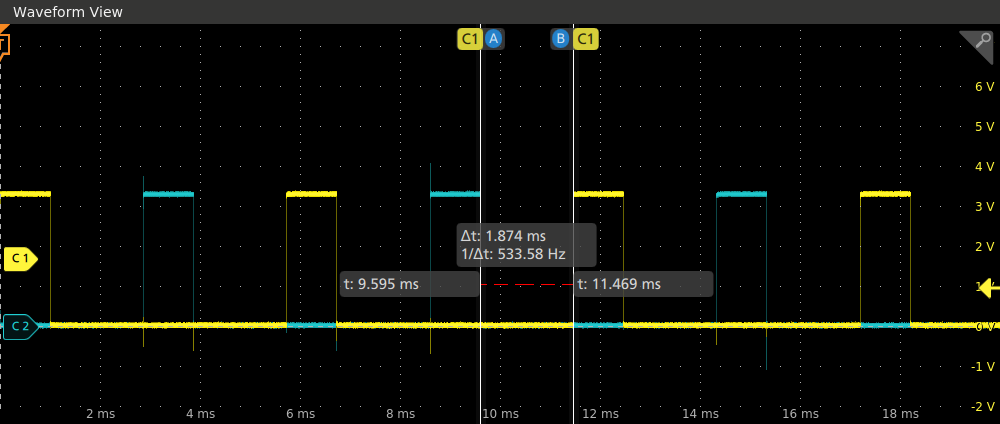
\includegraphics[width=0.9\textwidth]{assets/framework-value-wave.png}
%     \caption{\label{fig:internal-framework-value-wave}Internal benchmarking framework voltage measurement}

%   \end{minipage}\hfill
%   \begin{minipage}{0.45\textwidth}

%     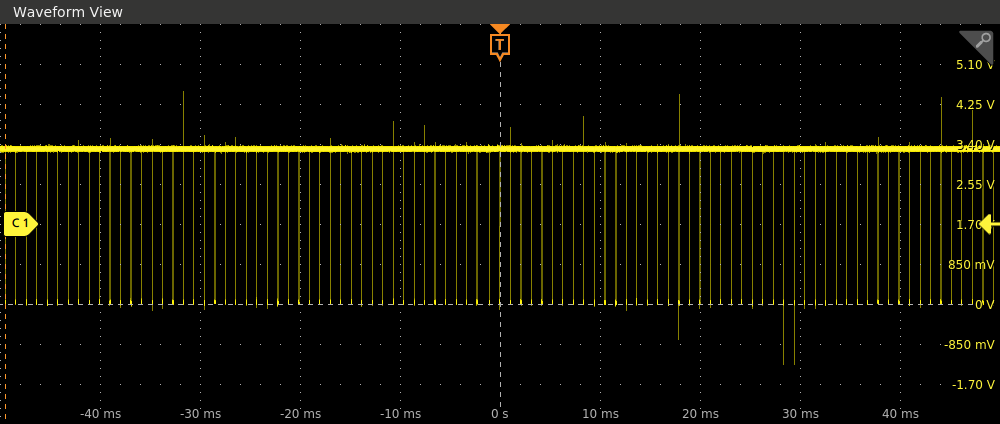
\includegraphics[width=0.9\textwidth]{assets/external-framework-value-wave.png}
%     \caption{\label{fig:external-framework-value-wave}External benchmarking framework voltage measurement}

%   \end{minipage}
% \end{figure}

% The table \ref{tab:frameworks-oscilloscope-comparison} shows a comparison of the real context switching time measured with the oscilloscope between the internal framework and the external one.

% \begin{table}[!ht]
%   \centering
%   \begin{tabular}{llllllll}
  & \multicolumn{7}{c}{Time ($\mu$s)}                                                      \\ \cline{2-8} 
  & \multicolumn{3}{c}{Internal framework} &  & \multicolumn{3}{c}{External framework} \\ \cline{2-4} \cline{6-8} 
  & \multicolumn{1}{c}{Mean} & Min  & Max  &  & Mean        & Min         & Max        \\ \cline{2-4} \cline{6-8} 
Context switching time & 1865                     & 1862 & 1866 &  & 14.87       & 14.79       & 14.97      \\
Duration of task 1     & 1003                     & 1003 & 1003 &  & 1003        & 1003        & 1003       \\
Duration of task 2     & 1003                     & 1003 & 1003 &  & 1003        & 1003        & 1003      
\end{tabular}
%   \caption{Context switching times and task durations measured with the oscilloscope using our internal and external benchmarking frameworks}
%   \label{tab:frameworks-oscilloscope-comparison}
% \end{table}

% \section{Discussions}

% \subsection{Internal benchmarking framework}

% By comparing with our reference measurement, the first assessment we can make is that our benchmarking framework does not compute the context switching time correctly.
% The framework measure a context switching time of 7812 $\mu$s where we expect a value of 14.68 $\mu$s.

% Second assessment we can make is that our framework add a huge overhead.
% When comparing the figure \ref{fig:measurement-value-wave} with the figure \ref{fig:internal-framework-value-wave}, the overhead is largely visible.
% By comparing the values measured by the oscilloscope, the reference measurement and the real context switching time while using our framework, we see that our framework add an overhead of 1850 $\mu$s.
% The table \ref{tab:measurements-comparison} shows this comparison.

% \begin{table}[!ht]
%   \centering
%   \begin{tabular}{lll}
%                         & \multicolumn{2}{c}{Time ($\mu$s)}                                     \\ \cline{2-3} 
%                         & \multicolumn{1}{c}{No framework} & Framework \\ \cline{2-3} 
%   From task 1 to task 2 & 14.68                                     & 1864                  \\
%   From task 2 to task 1 & 14.88                                     & 1865                  \\
%   Duration of task 1    & 1003                                      & 1003                  \\
%   Duration of task 2    & 1003                                      & 1003                 
%   \end{tabular}
%   \caption{Comparison of the oscilloscope measurements}
%   \label{tab:measurements-comparison}
% \end{table}

% \subsubsection{Limitations of the framework}
% As the results show, our framework suffers from several limitations.

% First, the devices can not compute the context switching time with enough precision.
% This lack of precision is due of the speed of the device clock that is not high enough.
% In our experiment, the Zolertia RE-MOTE used with Contiki could only use a timer with 128 ticks per second or 1 tick every 7812 $\mu$s.

% Second, our framework output its computed value through serial port.
% Printing out at least 32 characters for every context switch on the serial port even at 250 kbit/s took 1.2ms.
% One optimization could be to reduce the number of bits send or use a cache.

% \subsection{External benchmarking framework}

% The first thing we can see is that our external benchmarking framework is much more precise that our internal benchmarking framework.
% Even if the result does not match our excpectation, the results show an improvement.
% We went from a measurement error with a factor of more than 500 to a measurement error with a factor less than 2.

% Secondly, with the real context switching time measured at 14.87$\mu$s while our framework was on, our external benchmarking framework does not add an overhead.

% In conclusion, our external benchmarking framework is more precise than our internal benchmarking framework and does not add an overhead to the real context switching time.